\documentclass[a4paper,11pt]{article}

% Kodovani (cestiny) v dokumentu: utf-8
%\usepackage[cp1250]{inputenc}	% Omezena stredoevropska kodova stranka, pouze MSW.
\usepackage[utf8]{inputenc}	% Doporucujeme pouzivat UTF-8 (unicode).

\usepackage[margin=2cm]{geometry}
\newtoks\jmenopraktika \newtoks\jmeno \newtoks\datum
\newtoks\obor \newtoks\skupina \newtoks\rocnik \newtoks\semestr
\newtoks\cisloulohy \newtoks\jmenoulohy
\newtoks\tlak \newtoks\teplota \newtoks\vlhkost

\jmenopraktika={Fyzikální praktikum 3}
\jmeno={Lukáš Lejdar}
\datum={22. dubna 2025}
\obor={F}
\skupina={Út 14:00}

\cisloulohy={2}
\jmenoulohy={Určení měrného náboje elektronu}

%%%%%%%%%%% Uzitecne balicky:
\usepackage[czech]{babel}

\usepackage{graphicx}
\usepackage{amsmath}
\usepackage{xspace}
\usepackage{url}
\usepackage{indentfirst}
\usepackage{wrapfig}
\usepackage{xcolor}
\usepackage{subfig}
\usepackage{subcaption}
\usepackage{enumitem}
\usepackage{tikzsymbols}
\usepackage{newfloat}

\DeclareFloatingEnvironment[fileext=lof]{graph}
\captionsetup[graph]{labelformat=simple, labelsep=colon, name=Graf}

%%%%%% Zamezeni parchantu:
\widowpenalty 10000 \clubpenalty 10000 \displaywidowpenalty 10000
%%%%%% Parametry pro moznost vsazeni vetsiho poctu obrazku na stranku
\setcounter{topnumber}{3}	  % max. pocet floatu nahore (specifikace t)
\setcounter{bottomnumber}{3}	  % max. pocet floatu dole (specifikace b)
\setcounter{totalnumber}{6}	  % max. pocet floatu na strance celkem
\renewcommand\topfraction{0.9}	  % max podil stranky pro floaty nahore
\renewcommand\bottomfraction{0.9} % max podil stranky pro floaty dole
\renewcommand\textfraction{0.1}	  % min podil stranky, ktery musi obsahovat text
\intextsep=8mm \textfloatsep=8mm  %\intextsep pro ulozeni [h] floatu a \textfloatsep pro [b] or [t]

% Tecky za cisly sekci:
\renewcommand{\thesection}{\arabic{section}.}
\renewcommand{\thesubsection}{\thesection\arabic{subsection}.}
% Jednopismenna mezera mezi cislem a nazvem kapitoly:
\makeatletter \def\@seccntformat#1{\csname the#1\endcsname\hspace{1ex}} \makeatother
%
\newcommand{\vsn}[4]{\ensuremath{#1 =} #2(#3)\,#4}
\newcommand{\vrn}[6]{\ensuremath{#1 =} (#2 $\pm$ #3)\,#4 ($p=$ #5\,\%, $\nu=$ #6)}

\newcommand*\circled[1]{\tikz[baseline=(char.base)]{
		\node[shape=circle,draw,inner sep=1pt] (char) {#1};}}

%%%%%%%%%%%%%%%%%%%%%%%%%%%%%%%%%%%%%%%%%%%%%%%%%%%%%%%%%%%%%%%%%%%%%%%%%%%%%%%
% Zacatek dokumentu
%%%%%%%%%%%%%%%%%%%%%%%%%%%%%%%%%%%%%%%%%%%%%%%%%%%%%%%%%%%%%%%%%%%%%%%%%%%%%%%

\begin{document}

\thispagestyle{empty}

{
\begin{center}
\sf 
{\Large Ústav fyziky a technologií plazmatu Přírodovědecké fakulty Masarykovy univerzity} \\
\bigskip
{\huge \bfseries FYZIKÁLNÍ PRAKTIKUM} \\
\bigskip
{\Large \the\jmenopraktika}
\end{center}

\bigskip

\sf
\noindent
\setlength{\arrayrulewidth}{1pt}
\begin{tabular*}{\textwidth}{@{\extracolsep{\fill}} l l}
\large {\bfseries Zpracoval:}  \the\jmeno & \large  {\bfseries Naměřeno:} \the\datum\\[2mm]
\large  {\bfseries Obor:} \the\obor  \hspace{40mm}  {\bfseries Skupina:} \the\skupina %
&\large {\bfseries Testováno:}\\
\\
\hline
\end{tabular*}
}

\bigskip

{
\sf
\noindent \begin{tabular}{p{4cm} p{0.6\textwidth}}
\Large  Úloha č. {\bfseries \the\cisloulohy:} \par
\smallskip
&\Large \bfseries \the\jmenoulohy  \\[2mm]
\end{tabular}
}

\vskip1cm

\section{Úvod}

Cílem praktika je zjistit měřený náboj elektronu $ e / m $, tedy poměr mezi jeho nábojem a hmotností. Historicky byla tato veličina poprvé změřená Jhonem Thompsonem, který k tomu použil vychylování elektronového svazku pomocí elektromagnetického pole. Toto měření bude založené na podobném principu, konkrétně na pohybu elektronů v homogenním magnetickém poli. 

 
\section{Teorie}

Měrný náboj budeme měřit na elektronech vyletujících z rozžhavené katody do prostoru elektronky. Jejich počáteční energie je relativně malá, takže celková kinetická energie každého elektronu bude odpovídat urychlujícímu napětí $ U $  podle vztahu

\begin{equation}
e U = \frac{1}{2} m v^2,
\end{equation}

\noindent
kde $ e $  je náboj elektronů, $ m $  jejich hmotnost a $ v $ výstupní rychlost. Skleněná elektronka je naplněná vodíkem o tlaku $ P = 1 $ Pa, takže při pokojové teplotě $ T $ mají elektrony mnohem delší střední volnou dráhu, kterou můžeme přibližně spočítat podle 

\begin{equation}
\lambda = \frac{1}{n \sigma} = \frac{1}{ \sqrt{2}  \pi d^2}  \frac{k_b T}{P} \approx 1  \text{ cm}
\end{equation}

\noindent
kde odhad efektivního poloměru molekul vodíku je $ d \approx 0.3 $ nm a $ k_b $ je Boltzmanova konstanta. Po srážce s elektronem se vodíkové atomy excitují a při následné deexcitaci emitují viditelné záření, takže za sebou svazek elektronů nechá světelnou stopu. Celá elektronka se taky nachází uvnitř dvou Hemholtzových cívek, které v ní indukují příčné magnetické pole o indukci $ \vec{B} $. Síla $ \vec{F} $  působící na elektrony je podle Lorentzova vztahu vždy kolmá na rychlost elektronů 

\begin{equation}
\vec{F} = -e (\vec{v} \times \vec{B} )
\end{equation}

\noindent
a elektrony by se tak měli pohybovat po kružnici o poloměru $ R $. Z velikosti dostředivého zrychlení dostáváme vztah

\begin{equation}
\frac{ m v^2}{R} =  e v B
\end{equation}

\noindent
odkud už jde spočítat měrný náboj $ e / m $, pokud změříme indukci $ B $, výstupní rychlost $ v $ a poloměr $ R $. Vyjádřením ze vztahů (1) a (4) dostáváme 

\begin{equation}
\frac{e}{m} =  \frac{2 U}{ R^2 B^2} 
\end{equation}

\newpage

\section{Výsledky měření}

Celá soustava se skládá z jedné katody uvnitř elektronky na které můžu regulovat napětí $ U $ a dvou cívek do kterých teče proud $ I $. Před měřením je potřeba zjistit jaká magnetická indukce $ B(I) $ je indukovaná v místech elektronky v závislost na proudu tekoucích cívkami. Tyto hodnoty jsem už dostal a uvedl je v tabulce 1.


\begin{table}[h]
    \centering
    \begin{tabular}{| c | c c c c c c c c |}
        \hline 
    $ I $ (A) & 0.50 & 0.70 & 0.90 & 1.00 & 1.20 & 1.40 & 1.60 & 1.80 \\
    \hline
    $ B $ (mT) & 0.36 & 0.52 & 0.68 & 0.74 & 0.90 & 1.06 & 1.20 & 1.36 \\
    \hline
    \end{tabular}

    \caption{Závislost magnetické indukce na proudu tekoucím cívkami.}
\end{table}

Při samotném měření jsem krokově měnil proud a vždy doladil napětí tak, aby vzniklá kružnice byla co největší a odečtení jejího průměru $ D $ co nejpřesnější. K měření průměru sloužilo připevněné pravítko se dvěma jezdci, které byly nejdřív každý zvlášť posunutý do místa kde byly v zákrytu s kruhem elektronů a výsledný průměr se odečetl jako vzdálenost mezi nimi. Tímto způsobem naměřená data jsou uvedená v tabulce 2. Z nich je vykreslený graf závislosti $ 2U = f( \frac{D^2}{4} B^2) $ odkud podle vztahu (5) dostávám lineární regresí měrný náboj elektronu

\begin{equation}
\frac{e}{m} = -(1.65 \pm  0.03) \cdot 10^{11} \  \frac{\text{C}}{\text{kg}}
\end{equation}

\begin{table}[htpb]
    \begin{minipage}{.45\linewidth}
        \centering
        \begin{tabular}{| c c c c |}
            \hline
            $ I $ (A) & $ U $  (V) & $ D $ (cm) & $ B $  (mT) \\
            \hline
            0.74 &  -92.0 & 11.0 & 0.552 \\
            0.78 & -115.4 & 11.7 & 0.584 \\
            0.84 &  -98.2 & 11.5 & 0.632 \\
            0.94 & -129.5 & 10.5 & 0.704 \\
            1.06 & -144.0 & 10.4 & 0.788 \\
            1.18 & -158.7 & 10.1 & 0.884 \\
            1.18 & -178.4 & 11.3 & 0.884 \\
            1.32 & -185.9 & 09.6 & 0.996 \\
            1.32 & -216   & 10.1 & 0.996 \\
            1.42 & -250   & 10.1 & 1.074 \\
            1.48 & -277   & 10.3 & 1.116 \\
            1.63 & -303   & 10.0 & 1.224 \\
            1.76 & -303   & 08.9 & 1.328 \\
            2.01 & -303   & 08.1 & 1.528 \\
            \hline
        \end{tabular}
        \caption{Změřené poloměry kruhu elektronů při proudu cívkami a proudu a napětí na katodě.}
    \end{minipage} 
    \hfill
    \begin{minipage}{.5\linewidth}
        \centering
        \resizebox{\textwidth}{!}{ % GNUPLOT: LaTeX picture with Postscript
\begingroup
  \makeatletter
  \providecommand\color[2][]{%
    \GenericError{(gnuplot) \space\space\space\@spaces}{%
      Package color not loaded in conjunction with
      terminal option `colourtext'%
    }{See the gnuplot documentation for explanation.%
    }{Either use 'blacktext' in gnuplot or load the package
      color.sty in LaTeX.}%
    \renewcommand\color[2][]{}%
  }%
  \providecommand\includegraphics[2][]{%
    \GenericError{(gnuplot) \space\space\space\@spaces}{%
      Package graphicx or graphics not loaded%
    }{See the gnuplot documentation for explanation.%
    }{The gnuplot epslatex terminal needs graphicx.sty or graphics.sty.}%
    \renewcommand\includegraphics[2][]{}%
  }%
  \providecommand\rotatebox[2]{#2}%
  \@ifundefined{ifGPcolor}{%
    \newif\ifGPcolor
    \GPcolorfalse
  }{}%
  \@ifundefined{ifGPblacktext}{%
    \newif\ifGPblacktext
    \GPblacktexttrue
  }{}%
  % define a \g@addto@macro without @ in the name:
  \let\gplgaddtomacro\g@addto@macro
  % define empty templates for all commands taking text:
  \gdef\gplbacktext{}%
  \gdef\gplfronttext{}%
  \makeatother
  \ifGPblacktext
    % no textcolor at all
    \def\colorrgb#1{}%
    \def\colorgray#1{}%
  \else
    % gray or color?
    \ifGPcolor
      \def\colorrgb#1{\color[rgb]{#1}}%
      \def\colorgray#1{\color[gray]{#1}}%
      \expandafter\def\csname LTw\endcsname{\color{white}}%
      \expandafter\def\csname LTb\endcsname{\color{black}}%
      \expandafter\def\csname LTa\endcsname{\color{black}}%
      \expandafter\def\csname LT0\endcsname{\color[rgb]{1,0,0}}%
      \expandafter\def\csname LT1\endcsname{\color[rgb]{0,1,0}}%
      \expandafter\def\csname LT2\endcsname{\color[rgb]{0,0,1}}%
      \expandafter\def\csname LT3\endcsname{\color[rgb]{1,0,1}}%
      \expandafter\def\csname LT4\endcsname{\color[rgb]{0,1,1}}%
      \expandafter\def\csname LT5\endcsname{\color[rgb]{1,1,0}}%
      \expandafter\def\csname LT6\endcsname{\color[rgb]{0,0,0}}%
      \expandafter\def\csname LT7\endcsname{\color[rgb]{1,0.3,0}}%
      \expandafter\def\csname LT8\endcsname{\color[rgb]{0.5,0.5,0.5}}%
    \else
      % gray
      \def\colorrgb#1{\color{black}}%
      \def\colorgray#1{\color[gray]{#1}}%
      \expandafter\def\csname LTw\endcsname{\color{white}}%
      \expandafter\def\csname LTb\endcsname{\color{black}}%
      \expandafter\def\csname LTa\endcsname{\color{black}}%
      \expandafter\def\csname LT0\endcsname{\color{black}}%
      \expandafter\def\csname LT1\endcsname{\color{black}}%
      \expandafter\def\csname LT2\endcsname{\color{black}}%
      \expandafter\def\csname LT3\endcsname{\color{black}}%
      \expandafter\def\csname LT4\endcsname{\color{black}}%
      \expandafter\def\csname LT5\endcsname{\color{black}}%
      \expandafter\def\csname LT6\endcsname{\color{black}}%
      \expandafter\def\csname LT7\endcsname{\color{black}}%
      \expandafter\def\csname LT8\endcsname{\color{black}}%
    \fi
  \fi
    \setlength{\unitlength}{0.0500bp}%
    \ifx\gptboxheight\undefined%
      \newlength{\gptboxheight}%
      \newlength{\gptboxwidth}%
      \newsavebox{\gptboxtext}%
    \fi%
    \setlength{\fboxrule}{0.5pt}%
    \setlength{\fboxsep}{1pt}%
    \definecolor{tbcol}{rgb}{1,1,1}%
\begin{picture}(8640.00,5040.00)%
    \gplgaddtomacro\gplbacktext{%
      \csname LTb\endcsname%%
      \put(682,151){\makebox(0,0)[r]{\strut{}$10$}}%
      \put(682,929){\makebox(0,0)[r]{\strut{}$20$}}%
      \put(682,1707){\makebox(0,0)[r]{\strut{}$30$}}%
      \put(682,2485){\makebox(0,0)[r]{\strut{}$40$}}%
      \put(682,3263){\makebox(0,0)[r]{\strut{}$50$}}%
      \put(682,4041){\makebox(0,0)[r]{\strut{}$60$}}%
      \put(682,4819){\makebox(0,0)[r]{\strut{}$70$}}%
      \put(1726,-69){\makebox(0,0){\strut{}$2000$}}%
      \put(2812,-69){\makebox(0,0){\strut{}$2500$}}%
      \put(3899,-69){\makebox(0,0){\strut{}$3000$}}%
      \put(4985,-69){\makebox(0,0){\strut{}$3500$}}%
      \put(6071,-69){\makebox(0,0){\strut{}$4000$}}%
      \put(7157,-69){\makebox(0,0){\strut{}$4500$}}%
      \put(8243,-69){\makebox(0,0){\strut{}$5000$}}%
    }%
    \gplgaddtomacro\gplfronttext{%
      \csname LTb\endcsname%%
      \put(7256,4646){\makebox(0,0)[r]{\strut{}čidlo 1}}%
      \csname LTb\endcsname%%
      \put(7256,4426){\makebox(0,0)[r]{\strut{}čidlo 2}}%
      \csname LTb\endcsname%%
      \put(7256,4206){\makebox(0,0)[r]{\strut{}čidlo 3}}%
      \csname LTb\endcsname%%
      \put(7256,3986){\makebox(0,0)[r]{\strut{}čidlo 4}}%
      \csname LTb\endcsname%%
      \put(7256,3766){\makebox(0,0)[r]{\strut{}fit}}%
      \csname LTb\endcsname%%
      \put(209,2485){\rotatebox{-270.00}{\makebox(0,0){\strut{}t $^{\circ} C$}}}%
      \put(4528,-399){\makebox(0,0){\strut{}$\tau$ [s]}}%
    }%
    \gplbacktext
    \put(0,0){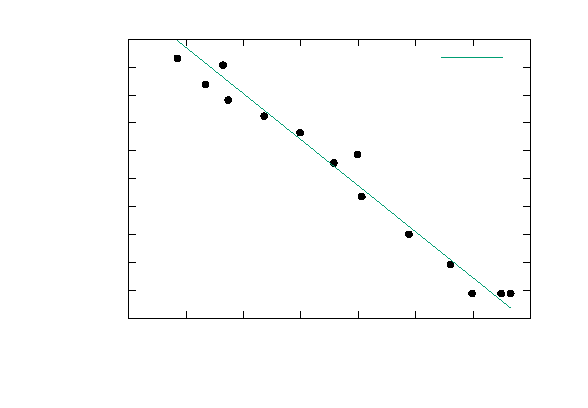
\includegraphics[width={432.00bp},height={252.00bp}]{mereni}}%
    \gplfronttext
  \end{picture}%
\endgroup
 }
        \captionsetup{type=graph}
        \caption{Závislost napětí $ 2U $ na druhé mocnině součinu poloměru kružnice s indukcí magnetického pole podle vztahu (5) }
    \end{minipage} 
\end{table}

\section{Závěr}

Z měření průměru kružnice opisované elektrony při známé rychlosti uvnitř homogenního magnetického pole jsem určil měrný náboj elektronu na $ e / m = -(1.65 \pm  0.03) \cdot 10^{11} \  \frac{\text{C}}{\text{kg}} $. Tabulková hodnota je $ e / m = -(1.7588) \cdot 10^{11} \  \frac{\text{C}}{\text{kg}} $,  takže měření přibližně vyšlo správně. Největší chybu do měření nejspíš zanáší měření poloměru kružnice, kterou nebylo jednoduché změřit přesně skrz elektronku.

\begin{thebibliography}{0}
\bibitem{tabulky} Návod k úloze ~\url{https://is.muni.cz/auth/el/sci/jaro2025/F4210/um/fp3-2_merny_naboj.pdf}.   
\end{thebibliography}

\end{document}
